    \hypertarget{random-forest---entrenamiento-del-algoritmo}{%
\section{Random Forest - Entrenamiento del algoritmo}\label{random-forest---entrenamiento-del-algoritmo}}

	Como se mencionó en el Marco Teórico \ref{sec:RF}, consta de un conjunto de árboles de decisión individuales, cada uno de los cuales se entrena mediante un procedimiento de arranque para seleccionar aleatoriamente muestras de los datos de entrenamiento originales. Esto significa que cada árbol se entrena con datos ligeramente diferentes. En cada árbol individual, las observaciones se propagan a través de bifurcaciones (nodos) que generan la estructura del árbol hasta llegar a un nodo terminal \cite{cien2001}.
	La BDD trabajada actualmente cuenta con:

    \begin{tcolorbox}[breakable, size=fbox, boxrule=1pt, pad at break*=1mm,colback=cellbackground, colframe=cellborder]
\prompt{In}{incolor}{53}{\boxspacing}
\begin{Verbatim}[commandchars=\\\{\}]
\PY{n+nb}{print}\PY{p}{(}\PY{l+s+s1}{\PYZsq{}}\PY{l+s+s1}{Existen }\PY{l+s+si}{\PYZob{}\PYZcb{}}\PY{l+s+s1}{ pacientes con }\PY{l+s+si}{\PYZob{}\PYZcb{}}\PY{l+s+s1}{ variables.}\PY{l+s+s1}{\PYZsq{}}\PY{o}{.}\PY{n}{format}\PY{p}{(}\PY{o}{*}\PY{n}{dataset}\PY{o}{.}\PY{n}{shape}\PY{p}{)}\PY{p}{)}
\PY{n+nb}{print}\PY{p}{(}\PY{l+s+s2}{\PYZdq{}}\PY{l+s+s2}{Existen}\PY{l+s+s2}{\PYZdq{}}\PY{p}{,} \PY{n}{dataset}\PY{o}{.}\PY{n}{size}\PY{p}{,} \PY{l+s+s2}{\PYZdq{}}\PY{l+s+s2}{elementos}\PY{l+s+s2}{\PYZdq{}}\PY{p}{)}
\end{Verbatim}
\end{tcolorbox}

    \begin{Verbatim}[commandchars=\\\{\}]
Existen 46 pacientes con 26 variables.
Existen 1196 elementos
    \end{Verbatim}

    \hypertarget{variable-categuxf3rica}{%
\subsection{Variable objetivo}\label{variable-categuxf3rica}}

 Al igual que en la sub sección \ref{NB:variable-categuxf3rica} se tomará la variable ``NIHSS\_alta\_ESTABLE\_O\_GRAVE'' con sus dos estados.
 
    \begin{tcolorbox}[breakable, size=fbox, boxrule=1pt, pad at break*=1mm,colback=cellbackground, colframe=cellborder]
\prompt{In}{incolor}{54}{\boxspacing}
\begin{Verbatim}[commandchars=\\\{\}]
\PY{c+c1}{\PYZsh{} variables objetivo e independientes:}
\PY{k+kn}{from} \PY{n+nn}{sklearn}\PY{n+nn}{.}\PY{n+nn}{model\PYZus{}selection} \PY{k+kn}{import} \PY{n}{train\PYZus{}test\PYZus{}split}

\PY{c+c1}{\PYZsh{} X son nuestras variables independientes}
\PY{n}{X} \PY{o}{=} \PY{n}{dataset}\PY{o}{.}\PY{n}{drop}\PY{p}{(}\PY{l+s+s1}{\PYZsq{}}\PY{l+s+s1}{NIHSS\PYZus{}alta\PYZus{}ESTABLE\PYZus{}O\PYZus{}GRAVE}\PY{l+s+s1}{\PYZsq{}}\PY{p}{,} \PY{n}{axis} \PY{o}{=} \PY{l+m+mi}{1}\PY{p}{)}

\PY{c+c1}{\PYZsh{} y es nuestra variable dependiente}
\PY{n}{y} \PY{o}{=} \PY{n}{dataset}\PY{p}{[}\PY{l+s+s1}{\PYZsq{}}\PY{l+s+s1}{NIHSS\PYZus{}alta\PYZus{}ESTABLE\PYZus{}O\PYZus{}GRAVE}\PY{l+s+s1}{\PYZsq{}}\PY{p}{]}

\PY{c+c1}{\PYZsh{} Uso de Skicit\PYZhy{}learn para dividir datos en conjuntos de entrenamiento y prueba }
\PY{c+c1}{\PYZsh{} División 75\PYZpc{} de datos para entrenamiento, 25\PYZpc{} de datos para test}
\PY{n}{X\PYZus{}train}\PY{p}{,} \PY{n}{X\PYZus{}test}\PY{p}{,} \PY{n}{y\PYZus{}train}\PY{p}{,} \PY{n}{y\PYZus{}test} \PY{o}{=} \PY{n}{train\PYZus{}test\PYZus{}split}\PY{p}{(}\PY{n}{X}\PY{p}{,} \PY{n}{y}\PY{p}{,} \PY{n}{test\PYZus{}size}\PY{o}{=}\PY{l+m+mf}{0.8}\PY{p}{,} \PY{n}{random\PYZus{}state}\PY{o}{=}\PY{l+m+mi}{0}\PY{p}{)}
\end{Verbatim}
\end{tcolorbox}

    \hypertarget{creaciuxf3n-del-modelo-y-entrenamiento}{%
\subsection{Creación del modelo y entrenamiento}\label{creaciuxf3n-del-modelo-y-entrenamiento}}

	De la misma manera que en la sub sección \ref{NB:creaciuxf3n-del-modelo-y-entrenamiento} crearemos el modelo.
	A continuación, entrenamos el modelo, pero sólo con los datos de entrenamiento. 

    \begin{tcolorbox}[breakable, size=fbox, boxrule=1pt, pad at break*=1mm,colback=cellbackground, colframe=cellborder]
\prompt{In}{incolor}{55}{\boxspacing}
\begin{Verbatim}[commandchars=\\\{\}]
\PY{k+kn}{from} \PY{n+nn}{sklearn}\PY{n+nn}{.}\PY{n+nn}{ensemble} \PY{k+kn}{import} \PY{n}{RandomForestClassifier}

\PY{c+c1}{\PYZsh{} Creamos el modelo de Bosque Aleatorio (y configuramos el número máximo de nodos\PYZhy{}hoja)}
\PY{n}{rfc} \PY{o}{=} \PY{n}{RandomForestClassifier}\PY{p}{(}\PY{n}{criterion} \PY{o}{=} \PY{l+s+s1}{\PYZsq{}}\PY{l+s+s1}{gini}\PY{l+s+s1}{\PYZsq{}}\PY{p}{,} \PY{n}{random\PYZus{}state}\PY{o}{=}\PY{l+m+mi}{0}\PY{p}{)}
\PY{n}{rfc}\PY{o}{.}\PY{n}{fit}\PY{p}{(}\PY{n}{X\PYZus{}train}\PY{p}{,} \PY{n}{y\PYZus{}train}\PY{p}{)}
\end{Verbatim}
\end{tcolorbox}

            \begin{tcolorbox}[breakable, size=fbox, boxrule=.5pt, pad at break*=1mm, opacityfill=0]
\prompt{Out}{outcolor}{55}{\boxspacing}
\begin{Verbatim}[commandchars=\\\{\}]
RandomForestClassifier(random\_state=0)
\end{Verbatim}
\end{tcolorbox}
        
    \hypertarget{estructura-del-uxe1rbol-creado}{%
\subsubsection{Estructura del árbol creado}\label{estructura-del-uxe1rbol-creado}}

    \begin{tcolorbox}[breakable, size=fbox, boxrule=1pt, pad at break*=1mm,colback=cellbackground, colframe=cellborder]
\prompt{In}{incolor}{56}{\boxspacing}
\begin{Verbatim}[commandchars=\\\{\}]
\PY{c+c1}{\PYZsh{} Import tools needed for visualization}
\PY{k+kn}{from} \PY{n+nn}{sklearn}\PY{n+nn}{.}\PY{n+nn}{tree} \PY{k+kn}{import} \PY{n}{export\PYZus{}graphviz}
\PY{k+kn}{import} \PY{n+nn}{pydot}

\PY{c+c1}{\PYZsh{} Pull out one tree from the forest}
\PY{n}{tree} \PY{o}{=} \PY{n}{rfc}\PY{o}{.}\PY{n}{estimators\PYZus{}}\PY{p}{[}\PY{l+m+mi}{5}\PY{p}{]}
\PY{n+nb}{print}\PY{p}{(}\PY{l+s+s1}{\PYZsq{}}\PY{l+s+s1}{The depth of this tree is:}\PY{l+s+s1}{\PYZsq{}}\PY{p}{,} \PY{n}{tree}\PY{o}{.}\PY{n}{tree\PYZus{}}\PY{o}{.}\PY{n}{max\PYZus{}depth}\PY{p}{)}

\PY{c+c1}{\PYZsh{} Export the image to a dot file}
\PY{n}{export\PYZus{}graphviz}\PY{p}{(}\PY{n}{tree}\PY{p}{,} \PY{n}{out\PYZus{}file} \PY{o}{=} \PY{l+s+s1}{\PYZsq{}}\PY{l+s+s1}{randomForestClassification.dot}\PY{l+s+s1}{\PYZsq{}}\PY{p}{,} \PY{n}{feature\PYZus{}names} \PY{o}{=} \PY{n}{feature\PYZus{}list}\PY{p}{,} \PY{n}{rounded} \PY{o}{=} \PY{k+kc}{True}\PY{p}{,} \PY{n}{precision} \PY{o}{=} \PY{l+m+mi}{1}\PY{p}{)}

\PY{c+c1}{\PYZsh{} Use dot file to create a graph}
\PY{p}{(}\PY{n}{graph}\PY{p}{,} \PY{p}{)} \PY{o}{=} \PY{n}{pydot}\PY{o}{.}\PY{n}{graph\PYZus{}from\PYZus{}dot\PYZus{}file}\PY{p}{(}\PY{l+s+s1}{\PYZsq{}}\PY{l+s+s1}{randomForestClassification.dot}\PY{l+s+s1}{\PYZsq{}}\PY{p}{)}

\PY{c+c1}{\PYZsh{} Write graph to a png file}
\PY{n}{graph}\PY{o}{.}\PY{n}{write\PYZus{}png}\PY{p}{(}\PY{l+s+s1}{\PYZsq{}}\PY{l+s+s1}{randomForestClassification.png}\PY{l+s+s1}{\PYZsq{}}\PY{p}{)}\PY{p}{;} 
\end{Verbatim}
\end{tcolorbox}

    \begin{Verbatim}[commandchars=\\\{\}]
The depth of this tree is: 4
    \end{Verbatim}
%%%%%%%%%%%%%%%%%%%%%%%%%%%%%%%%%%%%%%%%%%%%%%%%%%%%%%%%%%%%%%%%%%%%%%%%%%%%%%%
\begin{figure}
	\centering
	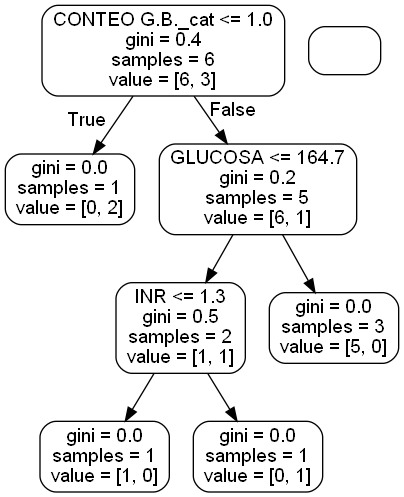
\includegraphics[scale=0.6]{Random Forest - Bosque Aleatorio/randomForestClassification.png} 
	\caption{Random Forest}
\end{figure}
%%%%%%%%%%%%%%%%%%%%%%%%%%%%%%%%%%%%%%%%%%%%%%%%%%%%%%%%%%%%%%%%%%%%%%%%%%%%%%%
    \hypertarget{predicciones-sobre-los-datos-de-prueba-y-muxe9tricas-de-rendimiento}{%
\subsection{Predicciones sobre los datos de prueba y métricas de rendimiento}\label{predicciones-sobre-los-datos-de-prueba-y-muxe9tricas-de-rendimiento}}

	Del mismo modo que en la sub sección \ref{NB:predicciones-sobre-los-datos-de-prueba-y-muxe9tricas-de-rendimiento} mostraremos las métricas del modelo en el entrenemiento.

    \begin{tcolorbox}[breakable, size=fbox, boxrule=1pt, pad at break*=1mm,colback=cellbackground, colframe=cellborder]
\prompt{In}{incolor}{57}{\boxspacing}
\begin{Verbatim}[commandchars=\\\{\}]
\PY{c+c1}{\PYZsh{} Predicción Entrenamiento }
\PY{n}{prediccionEntreno} \PY{o}{=} \PY{n}{rfc}\PY{o}{.}\PY{n}{predict}\PY{p}{(}\PY{n}{X\PYZus{}train}\PY{p}{)}

\PY{c+c1}{\PYZsh{} Predicción Tests}
\PY{n}{prediccionTests} \PY{o}{=} \PY{n}{rfc}\PY{o}{.}\PY{n}{predict}\PY{p}{(}\PY{n}{X\PYZus{}test}\PY{p}{)}
\end{Verbatim}
\end{tcolorbox}

    \begin{tcolorbox}[breakable, size=fbox, boxrule=1pt, pad at break*=1mm,colback=cellbackground, colframe=cellborder]
\prompt{In}{incolor}{58}{\boxspacing}
\begin{Verbatim}[commandchars=\\\{\}]
\PY{k+kn}{from} \PY{n+nn}{sklearn} \PY{k+kn}{import} \PY{n}{metrics}

\PY{n+nb}{print}\PY{p}{(}\PY{l+s+s2}{\PYZdq{}}\PY{l+s+s2}{Entrenamiento \PYZhy{} Presición :}\PY{l+s+s2}{\PYZdq{}}\PY{p}{,} \PY{n}{metrics}\PY{o}{.}\PY{n}{accuracy\PYZus{}score}\PY{p}{(}\PY{n}{y\PYZus{}train}\PY{p}{,} \PY{n}{prediccionEntreno}\PY{p}{)}\PY{p}{)}
\PY{n+nb}{print}\PY{p}{(}\PY{l+s+s2}{\PYZdq{}}\PY{l+s+s2}{Entrenamiento \PYZhy{} Reporte de clasificación:}\PY{l+s+se}{\PYZbs{}n}\PY{l+s+s2}{\PYZdq{}}\PY{p}{,} \PY{n}{metrics}\PY{o}{.}\PY{n}{classification\PYZus{}report}\PY{p}{(}\PY{n}{y\PYZus{}train}\PY{p}{,} \PY{n}{prediccionEntreno}\PY{p}{)}\PY{p}{)}
\end{Verbatim}
\end{tcolorbox}

    \begin{Verbatim}[commandchars=\\\{\}]
Entrenamiento - Presición : 1.0
Entrenamiento - Reporte de clasificación:
               precision    recall  f1-score   support

           0       1.00      1.00      1.00         6
           1       1.00      1.00      1.00         3

    accuracy                           1.00         9
   macro avg       1.00      1.00      1.00         9
weighted avg       1.00      1.00      1.00         9

    \end{Verbatim}

    Con un total de 34 pacientes, el algoritmo en la fase de entrenamiento predice en forma global un 100\%. Por cada estado (0 y 1) la precisión de los datos de entrenamiento en el modelo tiene un valor de 100\% para ambos estados en predicción. La exhaustividad informa la cantidad de datos capaz de identificar y, en este caso, es de un 100\% en ambos estados. Finalmente, el F1 combina los valores de precisión y exhaustividad obteniéndose un 100\% en ambos estados.

    \hypertarget{matriz-de-confusiuxf3n}{%
\subsection{Matriz de Confusión}\label{matriz-de-confusiuxf3n}}

	En el apartado del Marco Teórico \ref{sec:mc} se definió los conceptos y utilización que tenía esta herramienta. Para mayor claridad, visualizaremos la matriz de confusión en forma de mapa de calor.

    \begin{tcolorbox}[breakable, size=fbox, boxrule=1pt, pad at break*=1mm,colback=cellbackground, colframe=cellborder]
\prompt{In}{incolor}{59}{\boxspacing}
\begin{Verbatim}[commandchars=\\\{\}]
\PY{k+kn}{from} \PY{n+nn}{matplotlib} \PY{k+kn}{import} \PY{n}{pyplot} \PY{k}{as} \PY{n}{plot}
\PY{k+kn}{from} \PY{n+nn}{mlxtend}\PY{n+nn}{.}\PY{n+nn}{plotting} \PY{k+kn}{import} \PY{n}{plot\PYZus{}confusion\PYZus{}matrix}
\PY{k+kn}{from} \PY{n+nn}{sklearn}\PY{n+nn}{.}\PY{n+nn}{metrics} \PY{k+kn}{import} \PY{n}{confusion\PYZus{}matrix}

\PY{n}{matriz} \PY{o}{=} \PY{n}{confusion\PYZus{}matrix}\PY{p}{(}\PY{n}{y\PYZus{}train}\PY{p}{,} \PY{n}{prediccionEntreno}\PY{p}{)}

\PY{n}{plot\PYZus{}confusion\PYZus{}matrix}\PY{p}{(}\PY{n}{conf\PYZus{}mat}\PY{o}{=}\PY{n}{matriz}\PY{p}{,} \PY{n}{figsize}\PY{o}{=}\PY{p}{(}\PY{l+m+mi}{6}\PY{p}{,}\PY{l+m+mi}{6}\PY{p}{)}\PY{p}{,} \PY{n}{show\PYZus{}normed}\PY{o}{=}\PY{k+kc}{False}\PY{p}{)}
\PY{n}{plot}\PY{o}{.}\PY{n}{tight\PYZus{}layout}\PY{p}{(}\PY{p}{)}
\end{Verbatim}
\end{tcolorbox}

\begin{center}
    	\begin{figure}[H]
	\centering
    \adjustimage{max size={0.5\linewidth}{0.9\paperheight}}{Random Forest - Bosque Aleatorio/output_93_0.png}
	\caption{Matriz de confusión de entrenamiento Random Forest}
	\label{fig:mcerf}
	\end{figure}
\end{center}
    
    En la matriz de confusión \ref{fig:mcerf}, los valores de la diagonal principal (0,0) = 20 y (1,1) = 14 corresponden a los valores estimados de forma correcta por el modelo, tanto los TP, como los TN. La otra diagonal, representa los casos en los que el modelo \textit{"se ha equivocado"}, según la matriz de confusión \ref{fig:mcelr} son (0,1) = 0 FP y (1,0) = 0 FN.
\par Respecto al ACV, el modelo identificó a 20 pacientes que poseen un buen pronóstico (estable) y 14 pacientes que poseen un pronóstico no tan favorable, según la variable objetivo detallada en \ref{crear-columna-para-nihss_alta_estable_o_grave}.\\
